\documentclass[a4paper,11pt]{article}
\usepackage[margin=2.2cm]{geometry}
\usepackage{graphicx}
\usepackage{xcolor}
\usepackage{tikz}
\usetikzlibrary{arrows.meta,positioning}
\definecolor{RossNavy}{HTML}{17324D}
\definecolor{RossBlue}{HTML}{416D9B}
\definecolor{RossGray}{HTML}{AAB5BF}
\colorlet{RossPaleBlue}{RossBlue!8}
\colorlet{RossPaleGray}{RossGray!13}
\tikzset{
  rossbox/.style={draw=RossNavy,line width=0.85pt,rounded corners=2pt,
    minimum height=5.0cm,inner sep=4pt,align=center,font=\sffamily\normalsize},
  rossflow/.style={-Latex,line width=1.05pt,draw=RossNavy}
}
\begin{document}
\section{Framework for Mission 1}
\begin{figure}[htbp]
\centering
\resizebox{\linewidth}{!}{%
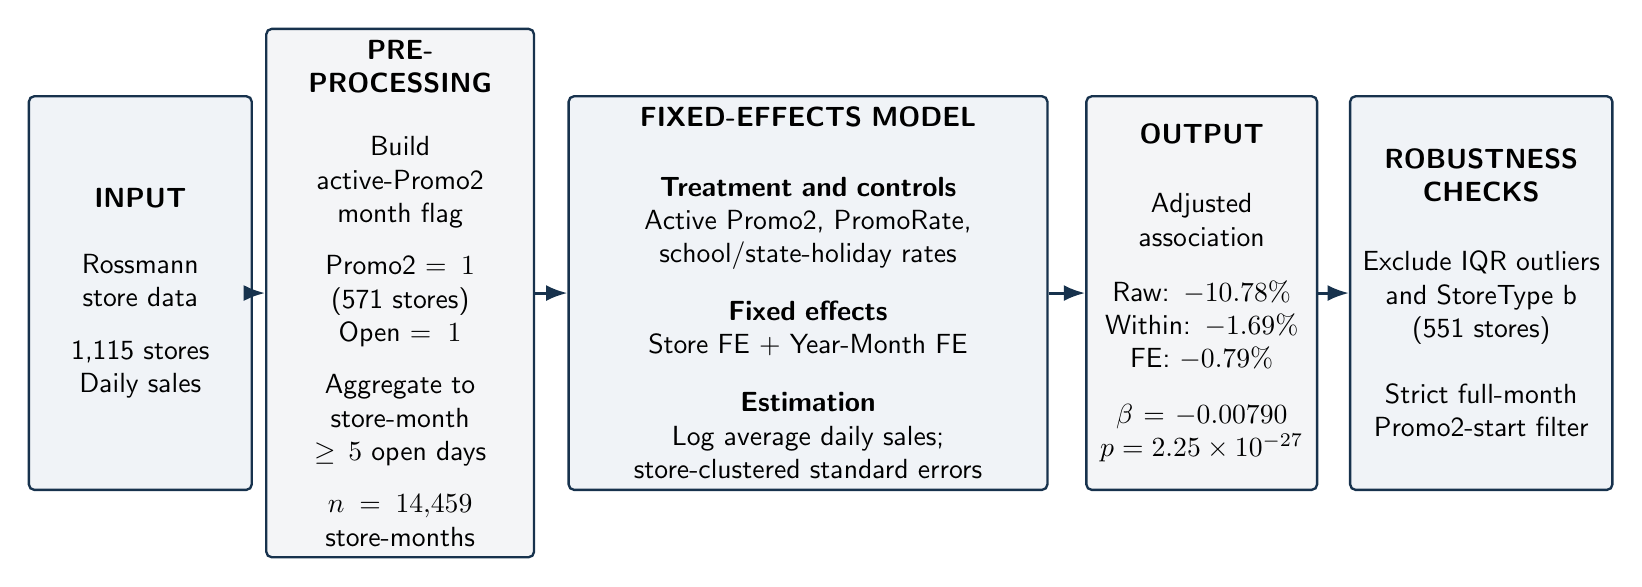
\begin{tikzpicture}
\node[rossbox,fill=RossPaleBlue,text width=2.55cm] (mi) at (0,0) {
  \textbf{INPUT}\\[12pt]
  Rossmann store data\\[7pt]
  1,115 stores\\Daily sales
};
\node[rossbox,fill=RossPaleGray,text width=3.12cm] (mp) at (3.30,0) {
  \textbf{PRE-PROCESSING}\\[11pt]
  Build\\active-Promo2 month flag\\[7pt]
  Promo2 $=1$ (571 stores)\\Open $=1$\\[7pt]
  Aggregate to store-month\\$\geq 5$ open days\\[7pt]
  $n=14{,}459$ store-months
};
\node[rossbox,fill=RossPaleBlue,text width=5.8cm] (mm) at (8.48,0) {
  \textbf{FIXED-EFFECTS MODEL}\\[13pt]
  \textbf{Treatment and controls}\\
  Active Promo2, PromoRate,\\school/state-holiday rates\\[9pt]
  \textbf{Fixed effects}\\
  Store FE + Year-Month FE\\[9pt]
  \textbf{Estimation}\\
  Log average daily sales;\\store-clustered standard errors
};
\node[rossbox,fill=RossPaleGray,text width=2.65cm] (mo) at (13.48,0) {
  \textbf{OUTPUT}\\[13pt]
  Adjusted association\\[8pt]
  Raw: $-10.78\%$\\
  Within: $-1.69\%$\\
  FE: $-0.79\%$\\[8pt]
  $\beta=-0.00790$\\
  $p=2.25\times10^{-27}$
};
\node[rossbox,fill=RossPaleBlue,text width=3.05cm] (mc) at (17.03,0) {
  \textbf{ROBUSTNESS CHECKS}\\[13pt]
  Exclude IQR outliers\\and StoreType b\\(551 stores)\\[12pt]
  Strict full-month\\Promo2-start filter
};
\draw[rossflow] (mi.east)--(mp.west);
\draw[rossflow] (mp.east)--(mm.west);
\draw[rossflow] (mm.east)--(mo.west);
\draw[rossflow] (mo.east)--(mc.west);
\end{tikzpicture}%
}
\caption{Mission 1 framework for evaluating the adjusted association between active Promo2 months and sales.}
\label{fig:mission1_framework}
\end{figure}

\clearpage
\section{Framework for Mission 2}
\begin{figure}[htbp]
\centering
\resizebox{\linewidth}{!}{%
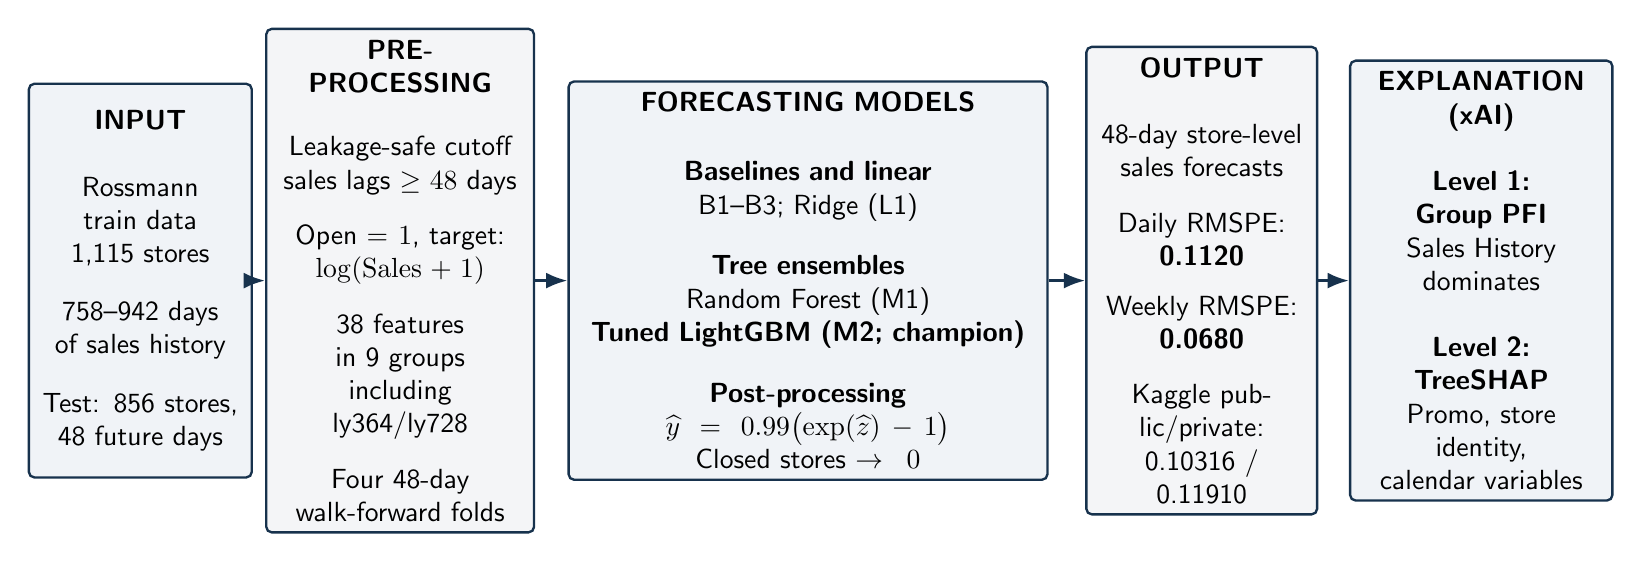
\begin{tikzpicture}
\node[rossbox,fill=RossPaleBlue,text width=2.55cm] (ti) at (0,0) {
  \textbf{INPUT}\\[12pt]
  Rossmann train data\\1,115 stores\\[9pt]
  758--942 days\\of sales history\\[9pt]
  Test: 856 stores,\\48 future days
};
\node[rossbox,fill=RossPaleGray,text width=3.12cm] (tp) at (3.30,0) {
  \textbf{PRE-PROCESSING}\\[11pt]
  Leakage-safe cutoff\\sales lags $\geq 48$ days\\[8pt]
  Open $=1$, target: \\$\log(\mathrm{Sales}+1)$\\[8pt]
  38 features in 9 groups\\including ly364/ly728\\[8pt]
  Four 48-day walk-forward folds
};
\node[rossbox,fill=RossPaleBlue,text width=5.8cm] (tm) at (8.48,0) {
  \textbf{FORECASTING MODELS}\\[13pt]
  \textbf{Baselines and linear}\\B1--B3; Ridge (L1)\\[10pt]
  \textbf{Tree ensembles}\\Random Forest (M1)\\\textbf{Tuned LightGBM (M2; champion)}\\[10pt]
  \textbf{Post-processing}\\$\widehat{y}=0.99\bigl(\exp(\widehat{z})-1\bigr)$\\Closed stores $\rightarrow 0$
};
\node[rossbox,fill=RossPaleGray,text width=2.65cm] (to) at (13.48,0) {
  \textbf{OUTPUT}\\[12pt]
  48-day store-level\\sales forecasts\\[8pt]
  Daily RMSPE:\\\textbf{0.1120}\\[6pt]
  Weekly RMSPE:\\\textbf{0.0680}\\[8pt]
  Kaggle public/private:\\0.10316 / 0.11910
};
\node[rossbox,fill=RossPaleBlue,text width=3.05cm] (te) at (17.03,0) {
  \textbf{EXPLANATION (xAI)}\\[12pt]
  \textbf{Level 1: Group PFI}\\Sales History dominates\\[12pt]
  \textbf{Level 2: TreeSHAP}\\Promo, store identity,\\calendar variables
};
\draw[rossflow] (ti.east)--(tp.west);
\draw[rossflow] (tp.east)--(tm.west);
\draw[rossflow] (tm.east)--(to.west);
\draw[rossflow] (to.east)--(te.west);
\end{tikzpicture}%
}
\caption{Mission 2 forecasting framework, leakage-safe preprocessing, walk-forward validation, and explainability.}
\label{fig:mission2_framework}
\end{figure}
\end{document}
